\documentclass[languages_and_machines.tex]{subfiles}
\begin{document}

\begin{frame}
  \frametitle{Turing Machine}

  \begin{block}{Definition}
    \textbf{Non-/Deterministic Turing Machine} := \begin{itemize}
    \item \(S\): set of states
    \item \(S_0 \in S\): initial state
    \item \(S_r, S_a \in S\): halt reject, halt accept state
    \item \(\Gamma\): tape alphabet
    \item \(b \in \Gamma\): blank symbol
    \item \(\Sigma \subseteq \Gamma \setminus \{b\}\): input alphabet
    \item \(f: S \times \Sigma \to S \times \Sigma \times \{R, L\}\): deterministic transition function
    \item \(f: S \times (\Sigma \cup \{\varepsilon\}) \to \powerset(S \times \Sigma \times \{R, L\})\): non-deterministic transition function
    \end{itemize}
  \end{block}
\end{frame}

\begin{frame}
  \frametitle{Turing Machine}

  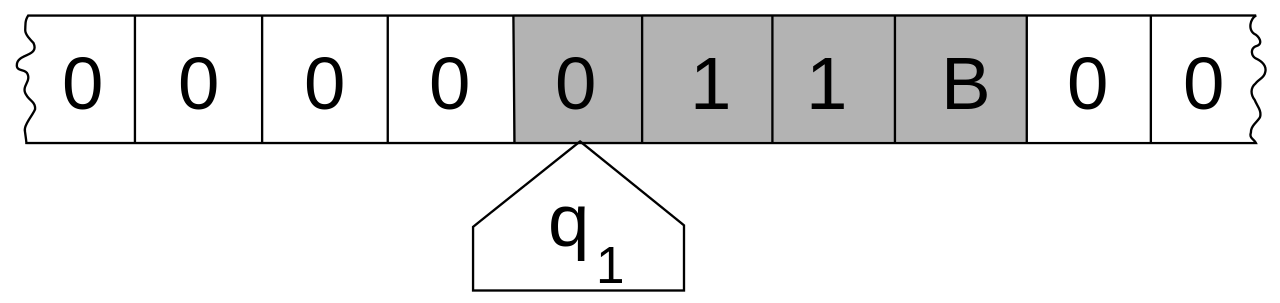
\includegraphics[width=1.0\textwidth]{turing_machine_1.png}

  {\tiny
    Figure from \href{https://commons.wikimedia.org/wiki/File:Turing_machine_2b.svg}{WikiMedia}
  }

  % \begin{tikzpicture}
  %   \begin{scope}[start chain=1 going right, node distance=-0.15mm]
  %     \node [on chain=1,tmtape,draw=none] {$\ldots$};
  %     \node [on chain=1,tmtape] {$A$};
  %     \node [on chain=1,tmtape] {0};
  %     \node [on chain=1,tmtape] {1};
  %     \node [on chain=1,tmtape,draw=red!50] {$1$};
  %     \node [on chain=1,tmtape,draw=none] {$\ldots$};
  %   \end{scope}
  % \end{tikzpicture}

\end{frame}

\begin{frame}
  \frametitle{Linear Bounded Turing Machine (LBTM)}

  Count possible 'complete-states' \(\lvert Q \rvert \lvert n \rvert \lvert \Sigma \rvert^{k \lvert n \rvert}\).

  \pause

  Finite number of complete-states, pigeon hole. If we hit the same complete-state twice, inf. loop.

  \pause

  Therefore inf. loops are detectable. Halting problem for LBTM is decidable.

  \pause

  Nobody knows if LBNTM \(\iff\) LB(D)TM

\end{frame}

\begin{frame}
  \frametitle{Context-Sensitive Grammar}

  CFG: \(A \to \alpha\)

  \pause

  CSG: \(\beta A \gamma \to \beta \alpha \gamma\) where \(\alpha \neq \varepsilon\)

  \pause

  \(\beta\)~\_~\(\gamma\) is the ``context''

  Repetition, optionals, nestedness\pause{}, with some memory

  \pause

  Note: Non-decreasing
\end{frame}

\begin{frame}
  \frametitle{LBNTM \(\iff\) CSL}

  Suppose \(\alpha \to \beta\) in a CSL with terminals \(\Sigma\) and non-terminals \(\Gamma\).

  \pause

  Let the tape alphabet be, \(\Gamma' = \Sigma \times (\Gamma \cup \{\Delta\})\).

  \pause

  Initially, tape has \(x_0 x_1 \dotsb x_n\). Convert to \((x_0, S), (x_1, \Delta) \dotsb (x_n, \Delta)\).

  \pause

  Simulate a CSG parse \(S \to \alpha \to \beta \to \dotsb \to x_0 x_1 \dotsb x_n\) in the \textit{second} coordinate in each cell.

  Accept if the first coordinate matches the second.

  \pause

  CSL's are non-decreasing, so linear bounded.

\end{frame}

\begin{frame}
  \frametitle{LBNTM \(\iff\) CSG}

  Construct CSG for given LBNTM:

  Let configuration := \(x_0 x_1 \dotsb x_{n-1} S_i x_n \dotsb x_k\)

  \pause

  Suppose \(\textcolor{green}{(S_i', x_n', L)} \in \textcolor{red}{f(S_i, x_n)}\). Then \(\textcolor{red}{S_i' x_{n-1} x_n'} \to \textcolor{green}{x_{n-1} S_i x_n}\).

  \pause

  This rule maps a configuration to the one configuration immediately prior. Example:

  \(x_0 x_1 \dotsb \textcolor{red}{S_i' x_{n-1} x_n'} \dotsb x_k\)

  \pause

  \(x_0 x_1 \dotsb \textcolor{green}{x_{n-1} S_i x_n} \dotsb x_k\)

  \pause

  We can work `backwards' to starting-tapes that the machine would accept!

  We will start with a rule that generates arbitrary finishing-tapes: \(b \to x_i b\) for \(x_i \in \Gamma\), in an accepting state \(S \to S_a b\).

\end{frame}

\begin{frame}
  \frametitle{CSL equivalents}

  \begin{itemize}
  \item Primitive recursive (composition, recursion counting down from \(n\))
    \pause
  \item Programming with only bounded for-loops and no recursion (see BlooP)
    \pause
  \item Kuroda Normal Form (\(AB \to CD, A \to BC, A \to B, A \to a\)) (exception for \(\varepsilon \in L\))
  \end{itemize}

\end{frame}

\end{document}
%%% Local Variables:
%%% mode: latex
%%% TeX-master: t
%%% End:
